\section{Introdução}
\label{sec:introducao}

Musicologia computacional é definida a grosso modo como o estudo de
música com a auxílio de programas de computador. Existem inúmeros
exemplos na literatura como o uso de vida artificial e algoritmos
evolutivos para estudar a evolução de ritmos e sistemas emocionais
\cite{coutinho05:conputational}, o uso de técnicas de mineração de
dados e aprendizado de máquina \cite{hartmann07:interactive}, e o
reconhecimento de estilos musicais \note{cita Kranenburg}. Alguns
artigos discutem o papel da computação na musicologia
\cite{kugel92:beyond,honing04:comeback,cook05:towards}.

Neste trabalho apresentamos o estudo de âmbitos, cruzamento de vozes,
quintas e oitavas consecutivas, acordes de sexta aumentada, resoluções
de sétimas, e estudo das cadências finais em 366 dos 371 corais de
Bach na edição de Riemenschneider \cite{bach41:371}. Cinco corais
ficaram de fora por problemas na conversão de MIDI para Lilypond (ver
seção \ref{sec:metodologia}). \cite{kostka.ea00:tonal} foi usado como
livro-texto base para comparações de procedimentos musicais usuais em
classes de harmonia. Neste trabalho o livro é referido no singular por
KP.

\section{Metodologia}
\label{sec:metodologia}

Todo o trabalho descrito neste artigo foi desenvolvido usando o
sistema \rameau{}\footnote{Está descrito em outro trabalho do autor, a
  citação foi removida por anonimato e será acrescentada na ocasião da
  publicação.} para análise automática de harmonia e extração de
informação musical. \rameau{} é um framework para implementação de
algoritmos de análise harmônica de partituras simbólicas. As
partituras são guardadas em arquivos no formato Lilypond
\cite{nienhuys.ea08:lilypond}, que permite diferenciação de notas
enarmônicas e geração de partituras bem tipografadas. As notas são
extraídas das partituras e apresentadas a uma rede neural, que associa
cada conjunto de notas a um acorde. Para coletar os dados usados neste
artigo \rameau{} foi estendido para realizar operações comuns de
musicologia como detecção de cruzamentos, quintas ou oitavas
consecutivas, cadências frequentes, etc.

Todos esses métodos de análise operam primeiro com a divisão da música
em \textbf{segmentos mínimos}, onde cada segmento mínimo é um conjunto
de notas que soam simultaneamente. Qualquer alteração nesse
conjunto---uma nota iniciando ou terminando, por exemplo---cria outro
segmento mínimo. Para detectar a resolução das sétimas, por exemplo,
\rameau{} primeiro procura todos os segmentos mínimos no coral
desejado que representam acordes com sétima e encontra, nesses
segmentos, as notas que são as sétimas dos acordes. Feito isso,
\rameau{} olha para o segmento imediatamente anterior para ver como
essas notas foram preparadas, olha para o segmento posterior para ver
se elas resolvem imediatamente, e formata os dados encontrados.

Além disso \rameau{} possui vários outros algoritmos para análise
harmônica, como o descrito em \cite{pardo.ea00:automated}, outras
redes neurais e classificadores de árvores de decisão e
k-vizinhos-mais-próximos. Atualmente \rameau{} está sendo estendido
para realizar análise funcional de qualquer peça tonal.

Os corais utilizados neste artigo foram convertidos de MIDI para o o
formato do Lilypond por uma ferramenta automática e depois corrigidos
manualmente para remover erros de enarmonia e notas incorretas. Usamos
gabaritos manuais de análise harmônica para validar os algoritmos de
análise, e o algoritmo escolhido para análise de cadências encontra
corretamente em torno de 98\% dos acordes\footnote{Idem.}.

\section{Análise}
\label{sec:analise}

\subsection{Âmbitos}
\label{sec:ambitos}

Os corais de Bach foram escritos para serem cantados por músicos
profissionais e não pela congregação \cite{bach41:371} \note{não gosto
  de ``escritos para serem cantados'' kroger: sugestoes?}. Esse fato
se reflete na textura, cruzamentos e no âmbito vocal usado nos corais.
A figura \ref{fig:ambito-kostka} mostra os âmbitos sugeridos por KP e
os utilizados por Bach nos corais analisados. Bach amplia o âmbito de
soprano e tenor em uma segunda maior ascendente, e o do contralto em
uma segunda maior descendente. A voz do baixo tem ampliação de uma
terça maior em ambas direções (comparando com KP). A tabela
\ref{tab:notas-extremas} lista os corais onde as notas mais agudas e
graves ocorrem em cada voz. Na figura \ref{fig:ambitos-alem} podemos
ver exemplos das notas mais graves e agudas na voz do baixo.

\begin{table}
\begin{center}
\begin{small}
\begin{sc}
  \begin{tabular}{r|p{4cm}p{4cm}}
    & nota mais aguda & nota mais grave \\ 
    \hline
    soprano &  116 254 282 298 331 334 &  186 034 050 068 075 223 049 070 100 165 185 197 214 325 348 158 175
    205 239 352 087 110 244 \\ \aroundspace
    contralto & 024 028 033 036 057 058 069 078 084 123 217 225 248 252 329 331 334
    354 359 &   345 186 \\ \aroundspace
    tenor &   024 043 074 083 151 156 224 248 263 264 273 276 281 329
    354 371 &   229 070 205 \\ \aroundspace
    baixo &   285 312 331 &   034 051 214 223 340 131 328 143 155 197 205 219 241 187 235 319 337
    240 070 075 165 175 239 
  \end{tabular}
  \caption{Corais com notas extremas}
  \label{tab:notas-extremas}
\end{sc}
\end{small}
\end{center}
\end{table}

\begin{figure}
  \centering
  \includegraphics[scale=2.5]{ambitos}
  \caption{Comparação de âmbito utilizado por Bach e definido por KP}
  \label{fig:ambito-kostka}
\end{figure}

\begin{figure}
  \centering
  \subfigure{\includegraphics[scale=2.5]{331-baixo-agudo}}
  \subfigure{\includegraphics[scale=2.5]{034-baixo-grave}}
  \caption{Notas mais grave e aguda do Baixo}
  \label{fig:ambitos-alem}
\end{figure}

\subsection{Cruzamento de vozes}
\label{sec:cruzamento-de-vozes}

Dos corais analisados, 209 tem cruzamentos entre as vozes (57\%). KP
sugere evitar cruzamentos, principalmente acima do soprano ou abaixo
do baixo. KP permite o cruzamento breve das linhas de contralto e
tenor se existir uma razão musical \cite[p. 79]{kostka.ea00:tonal}. De
fato, dos corais com cruzamento, o cruzamento mais comum é entre tenor
e contralto (65\%), mas o cruzamento entre tenor e baixo é quase tão
comum (60\%). O cruzamento entre contralto e soprano é menos frequente
(15\%), mas existente, contrariando a regra de não cruzar acima do
soprano. De qualquer forma, a grande maioria dos cruzamentos (85\%)
são curtos (nunca maiores que dois tempos). A análise de cruzamentos
mostra alguns exemplos interessantes: no coral 35 o contralto é a voz
mais grave por um breve período de tempo onde as vozes do tenor e
baixo estão acima da voz do contralto (figura
\ref{fig:035-cruzamento}), e no coral 290 existe um cruzamento
simultâneo do baixo com o tenor e do contralto com o soprano (figura
\ref{fig:290-66-74-cruzamento}).

\begin{figure}
  \centering
  \subfigure[Coral 35]{
    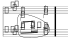
\includegraphics[scale=3]{035-16-20-cruzamento}
    \label{fig:035-cruzamento}
  }
  \subfigure[Coral 290]{
    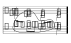
\includegraphics[scale=3]{290-66-74-cruzamento}
    \label{fig:290-66-74-cruzamento}
  }
  \subfigure[Coral 3]{
    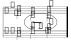
\includegraphics[scale=3]{003-38-42-cruzamento}
    \label{fig:003-38-42-cruzamento}
  }
  \caption{Cruzamentos entre vozes}
  \label{fig:coral-003}
\end{figure}

Os cruzamentos podem ser classificados em duas categorias; para evitar
quintas e oitavas consecutivas \ref{fig:003-38-42-cruzamento} e para
manter melhor condução de vozes \ref{fig:290-66-74-cruzamento}.
Contudo inúmeros cruzamentos poderiam ser evitados.

Em alguns corais com cruzamento entre baixo e tenor, por exemplo 29,
35 e 76, a edição usada sugere através de uma \textit{ossia} que as
notas do baixo sejam cantadas uma oitava abaixo para evitar o
cruzamento. Essa sugestão levanta a questão do porque Bach não
escreveu as notas nessa oitava em primeiro lugar.

\subsection{Quintas e oitavas consecutivas}
\label{sec:quintas-e-oitavas}

Apesar do uso de quintas e oitavas consecutivas ser relativamente
comum na escrita instrumental, seu uso constitui uma das regras mais
básicas a ser evitada no estudo de harmonia e contraponto. Dessa
maneira, é interessante verificar quantas oitavas e quintas
consecutivas existem nos corais de Bach. O número de oitavas e quintas
juntos é pouco representativo (4\%) em comparação com todos os corais
analisados. Existem 8 quintas e 7 oitavas consecutivas.

Algumas dessas quintas e oitavas ocorrem entre o último acorde de uma
frase e primeiro acorde da próxima, como nos corais 45 e 46 (quintas)
e 2, 89, e 279 (oitavas) (figura \ref{fig:279-oitava}). Uma possível
justificativa é a ``quebra'' de uma frase para outra. Contudo, a
maioria das quintas e oitavas consecutivas (9 no total) ocorre no meio
de frases. Todas as oitavas nessa categoria são uníssono--oitava ou
oitava--uníssono (figura \ref{fig:oitavas-e-unissonos}). Nenhuma
dessas oitavas é paralela, mas algumas das quintas são (corais 4, 46,
71, 266).

\begin{figure}
  \centering
  \subfigure[Coral 244]{
    \includegraphics[scale=5]{244-oitava}
    \label{fig:244-oitava}
  }
  \qquad
  \subfigure[Coral 279]{
    \includegraphics[scale=2.7]{279-oitava}
    \label{fig:279-oitava}
  }
  \qquad
  \subfigure[Coral 329]{
    \includegraphics[scale=2.8]{329-oitava}
    \label{fig:329-oitava}
  }
  \caption{Oitavas e uníssonos}
  \label{fig:oitavas-e-unissonos}
\end{figure}

\subsection{Acordes de sexta aumentada}
\label{sec:acordes-de-sexta}

Os corais apresentam exatamente três acordes de sexta aumentada e
exatamente um de cada tipo listado por KP: um acorde de sexta
aumentada alemã (coral 340), um acorde de sexta aumentada italiana
(coral 19), e um acorde de sexta aumentada francesa (coral 146). A
figura \ref{fig:sextas-aumentadas} mostra os três acordes. A falta de
um uso maior desses acordes nos corais sugere que nesses exemplos eles
são obtidos pelo resultado dos movimentos horizontais das vozes.

\begin{figure}
  \centering
  \subfigure[Sexta alemã (coral 340)]{
    \includegraphics[scale=3]{340-alema}
  }
  \subfigure[Sexta italiana (coral 19)]{
    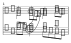
\includegraphics[scale=3]{019-1-9-italiana}
  }
  \subfigure[Sexta francesa (coral 146)]{
    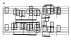
\includegraphics[scale=3]{146-20-27-francesa}
  }
  \caption{Sextas aumentadas}
  \label{fig:sextas-aumentadas}
\end{figure}

\subsection{Resoluções de sétimas}
\label{sec:setimas}

Encontramos nos corais de Bach um total de 6297 acordes com sétima e
verificamos o tratamento destas sétimas em segmentos adjacentes. Em
77\% dos casos as sétimas são resolvidas descendentemente e por grau
conjunto, ou seja, da maneira usual \cite[p. 207]{kostka.ea00:tonal}.
Nos acordes restantes em geral ocorre uma das quatro situações
seguintes:

\begin{enumerate}
\item A sétima não é resolvida e se transforma em nota do acorde
  seguinte, que pode ser a própria tétrade ou um novo acorde (16\% dos
  casos). Na figura \ref{fig:120-setima-koechlin} a sétima do acorde
  de bm7 se transforma na tônica do acorde seguinte.
\item No segmento seguinte à sétima, uma ou várias notas do acorde são
  tocadas antes da resolução, ou ainda a sétima desaparece. Na figura
  \ref{fig:049-setima-arpejo} há um arpejo antes da resolução.
\item O encadeamento das vozes por grau conjunto transforma a tétrade
  em uma espécie de acorde de passagem. Dessa forma a sétima perde sua
  função original (ver vozes circuladas na figura
  \ref{fig:015-setima-acorde-pass}).
\item A sétima é resolvida ascendentemente e cromaticamente, em geral
  como uma sensível local (menos de 1\% dos casos). Na figura
  \ref{fig:003-setima-asc-crom} a sétima ascende cromaticamente para a
  sensível da tônica do acorde seguinte.
\end{enumerate}

\begin{figure}
  \centering
  \subfigure[Sétima transformada em nota do acorde seguinte (coral 120)]{
    \includegraphics[scale=5]{120-setima-koechlin}
    \label{fig:120-setima-koechlin}
  }
  \subfigure[Arpejo antes da resolução (coral 49)]{
    \includegraphics[scale=3]{049-setima-arpejo}
    \label{fig:049-setima-arpejo}
  }
  \subfigure[Vozes de passagem (coral 15)]{
    \includegraphics[scale=5]{015-setima-acorde-pass}
    \label{fig:015-setima-acorde-pass}
  }
  \subfigure[Ascendente cromática (coral 3)]{
    \includegraphics[scale=3]{003-setima-asc-crom}
    \label{fig:003-setima-asc-crom}
  }
  \caption{Resoluções de sétima}
  \label{fig:setima-resol}
\end{figure}

\subsection{Cadências finais}
\label{sec:cadencias}

\rameau{} identifica 79\% das cadências finais (isso é, os três
últimos acordes diferentes) com o formato $x$ V I onde $x$ pode ser ii
(menor ou diminuto), IV (maior ou menor), V/V (dominante secundária),
ou I (maior ou menor) e último acorde pode ser maior ou menor.

A cadência mais comum é do tipo ii V I (36\%), seguida por I V I
(32\%). As cadências IV VI (6\%) e V/V V I (5\%) são estatisticamente
insignificantes. Apenas 3\% dos corais tem a cadência vii°/V V I, e
apenas 2\% do tipo viiø V I. \note{eu nao sei o que fazer aqui porque
  ``ii V I'' é generico, ii pode ser menor, diminuto, semi-dim, e I
  pode ser i. sugestoes? marcos: coloca uma nota de rodapé, explica
  isso e usa maiúsculas}

O algoritmo para analisar as cadências finais identifica de maneira
errada 16\% dos corais. Por exemplo, a cadência final do coral 362 é
I$^6_4$ V$_7$ I, mas o algoritmo interpreta a antecipação para a terça
do acorde final como um acorde menor do terceiro grau (iii). Além
disso, como o algoritmo sempre considera que o acorde final é de
tônica, ele classifica eroneamente os corais que terminam em acordes
diferentes da tônica, como os que terminam em meia-cadência.

\begin{figure}
  \centering
  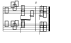
\includegraphics[scale=3]{341-99-104-cadencia}
  \caption{Cadência (coral 341)}
  \label{fig:cadencia}
\end{figure}

\section{Avaliação}
\label{sec:avaliacao}

\rameau{} verifica e interpreta corretamente dados como âmbitos e
cruzamento de vozes. Nós pudemos verificar, por exemplo, que mais da
metade dos corais possuem algum tipo de cruzamento.

Os acordes de sexta aumentada foram encontrados por um algoritmo que
busca pelo intervalo específico de sexta aumentada dentro de um
segmento. Isso significa que \rameau{} não encontrará um acorde de
sexta aumentada se ao notas que formam o intervalo de sexta aumentada
estiverem em segmentos diferentes (como em um arpejo). Isso não é
problema sério em uma composição no estilo coral, mas esperamos
resolver esse problema com a implementação de segmentação no sistema.

Neste artigo apresentamos apenas quintas e oitavas consecutivas entre
segmentos adjacentes. Apesar de \rameau{} possuir um algoritmo para
detectar quintas e oitavas consecutivas entre segmentos não
adjacentes, preferimos não incluir o resultado devido a necessidade de
refinamento do algoritmo.

A análise do tratamento de sétimas em segmentos adjacentes não
comporta os casos em que há acordes entre o aparecimento da sétima e a
sua resolução. O estudo de resolução de sétimas poderia ser
beneficiado se o algoritmo do \rameau{} analisasse o contexto em volta
do acorde de sétima de maneira dinâmica. Dessa maneira poderia se
fazer um estudo mais preciso de como sétimas são preparadas e
resolvidas.

Finalmente, o estudo de cadências pode ser melhorado com a
implementação da análise funcional no sistema.

\section{Conclusão e trabalhos futuros}
\label{sec:concl-e-trab}

Nesse artigo apresentamos um estudo de alguns elementos musicais nos
corais de Bach com o auxílio de sistema \rameau{}. Esse tipo de estudo
é interessante pela precisão e possibilidades de análise fornecidas.
Por exemplo, nossa análise indica que o soprano alcança a nota mais
grave em 23 corais. Essa informação pode ser usada para demonstrar
acordes em posição fechada. Em um outro exemplo, um professor de
harmonia pode selecionar trechos com resoluções específicas de sétima
para mostrar aos seus alunos. Naturalmente esses dados poderiam ser
extraídos manualmente, mas sem dúvida levaria um tempo enorme,
considerando que são mais de 30000 segmentos no total.

O maior desafio nesse tipo de análise é garantir que os dados de
entrada estejam 100\% corretos, especialmente em arquivos MIDI.
Infelizmente o número de erros é frequente \note{passos: o número é
  grande ou os erros são frequentes}. Uma possível solução seria a
criação de repositórios de arquivos musicais em formatos simbólicos
para análise. Esse arquivos seriam corrigidos sistematicamente por
pesquisadores de área. Alguns repositórios existem para composições no
formato kern (usado pelo Humdrum)\footnote{\url{kern.humdrum.net}} e
MuseData\footnote{\url{www.musedata.org}}. No final da nossa pesquisa
esperamos liberar um repositório com todos os corais de Bach no
formato do Lilypond corrigidos.

No futuro esperamos implementar segmentação e análise funcional no
sistema. Essa implementação resolverá a maioria dos problemas listados
na seção de avaliação.

%%% Local Variables: 
%%% mode: latex
%%% TeX-master: "musicologia-computacional-simples"
%%% End: 
